
	\subsection{Теорема Гильберта-90}

	Пусть $L/F$~--- конечное расширение Галуа. Тогда $G = \Gal(L/F)$ действует на $L$ и $L^*$ наделяется структурой $G$-модуля (как и $L^+$).

	\begin{theorem}[Hilbert-90] 
		Пусть $L/F$~--- конечное расширение Галуа. Тогда $H^{1}(G, L^*) = 0$.
	\end{theorem}

	Перед тем как доказывать эту теорему, сформулируем лемму Артина о линейной независимости характеров, которая поможет нам при доказательстве. 

	\begin{lemma}[Артин] 
		Пусть $K$~--- поле $H$~-- группа, а $\chi_1, \ldots, \chi_n\colon H \to K^*$~--- попарно-различные характеры. Пусть $a_1, \ldots, a_n \in K$ таковы, что 
		\[
			a_1 \chi_1 + \ldots + a_n \chi_n = 0.
		\]
		Тогда $a_1 = \ldots = a_n$.
	\end{lemma}

	\begin{proof}[Доказательство теоремы Гильберта-90]
		 Рассмотрим $f \in \Z^1(G, L^*)$ и рассмотрим 
		 \[
		 	\sum_{\sigma \in G} f(\sigma) \cdot \sigma.
		 \]
		 Это какая-то линейная комбинация попарно-различных характеров. Значит, по лемме Артина о независимости характеров найдётся $c \in L^*$ такое, что 
		 \[
		 	b = \sum_{\sigma \in G} f(\sigma) \cdot \sigma(c) \neq 0.
		 \]
		 Применим к этому равенству действие какого-то $\tau \in G$ и воспользуемся тем, что так как $f$~--- это 1 коцикл (т.е. скрученный гомоморфизм), $f(\tau \sigma) = f(\tau) \cdot \tau f(\sigma)$. Тогда 
		 \[
		 	\tau(b) = \sum_{\sigma \in G} (\tau f(\sigma)) (\tau \sigma(c)) = \sum_{x \in G} (f^{-1}(\tau)  f(\tau \sigma)) \cdot \tau\sigma(c) = f^{-1}(\tau) \sum_{\eta \in G} f(\eta) \eta(c) = f^{-1}(\tau) b.
		 \]
		 Таким образом, $f(\tau) = \frac{b}{\tau(b)}$, то есть $f$ является 1-кограницей и когомологии тривиальны. 
	\end{proof}

	\begin{remark}
		Исторически Гильберт доказал это только для циклических расширений (пользуясь тем, что все элементы это степени какого-то одного), а именно эту версию доказала Эмми Нётер. Но, стоит отметить, что доказательство проходит абсолютно такое же. Гильберт предпочитал понимать эту теорему в такой формулировке: если $x \in L^*$ таков, что $N x = 1$, то существует $b \in L^*$ такой, что $x = \frac{b}{\sigma(b)}$, где $\sigma$~--- образующая группы Галуа (у него группа Галуа была циклической). 
	\end{remark}


	Вообще говоря, в случае конечных полей эту теорему можно доказать и элементарным способом: 

	Пусть $L/F$~--- конечное расширение, $|F| = q = p^k$, $|L| = q^n$. Тогда у нас есть короткая точная последовательность 
	\[
		1 \to \Ker{N} \to L^* \to \Im{N} \to 1,
	\]
	откуда мы имеем 
	\[
		|L^*| = |\Im{N}| \cdot |\Ker{N}| \implies |\Im{N}| = \frac{q^n - 1}{|\Ker{N}|}
	\]
	\[	
		Nx = \prod_{\sigma \in \Gal(L/F)} \sigma x = \prod_{i = 0}^{n - 1} \sigma^i(x) = x^{1 + q + \ldots + q^{n - 1}}.
	\]
	Возьмём $x \in \Ker{N}$, тогда у нас есть уравнение 

	\[
		x^{1 + q + \ldots + q^{n - 1}} = 1.
	\]

	Количество корней этого уравнения не превосходит $1 + q + \ldots + q^{n - 1} = \frac{q^n - 1}{q - 1}$,  откуда 
	\[
		|\Ker{N}| \le \frac{q^n - 1}{q - 1}.
	\]
	Отсюда мы получаем неравенство 
	\[
		|\Im{N}| \ge q - 1 \implies |\Im{N}| = F^*.
	\]

	\section{Применения когомологий групп к теории чисел}

	\subsection{Вычисление $H^2(G, L^*)$}

	Пусть $K$~--- локальное поле, $L$~--- конечное расширение Галуа с группой Галуа $G = \Gal(L/K)$. Тогда, как мы помним, по теореме Гильберта-90:
	\[
		H^1(G, L^*) = 0.
	\]

	Вычислим $H^{2}(G, L^*) \cong \widehat{H}^2(G, L^*)$. Рассмотрим сначала случай неразветвлённого расширения (так как он проще). 

	\subsubsection{Случай неразветвлённого расширения}

	Как мы помним, в этом случае группа Галуа циклическая, а тогда по 2-периодичности когомологий циклической группы достаточно посчитать $\widehat{H}^0(G, L^*)$. По определению, 
	\[
		\widehat{H}^0(G, L^*) = \lr*{L^*}^G/N L^* \cong K^* / NL^*,
	\]
	так как просто по определению группы Галуа $\lr*{L^*}^G = K^*$. Как мы видели в параграфе про теорему Гильберта-90, в случае конечных полей такой фактор тривиален. Но, вообще говоря это не всегда так. 

	Таким образом, в случае неразветвлённого расширения мы имеем $H^2(G, L^*) \cong K^*/N L^*$. 

	Вспомним, что у нас есть такие фильтрации на кольцах $\cO_K$ и $\cO_L$:
	\[
		\cO_K = U_K = U_{K, 0} \supset U_{K, 1} \supset U_{K, 0} \supset \ldots 
	\]
	и аналогично для $\cO_L = U_L$, где 
	\[
		U_{L, i} = \{ x \in L \ \vert \ v_{L}(x - 1) \ge 1 \} = \{ 1 + \pi_L^i y \ \vert y \in \cO_L \} = 1 + \fm_L^i. 
	\]
	Так как расширение неразветвлено, $\pi_K = \pi_L \implies \fm_L = \fm_K$. Кроме того, мы вычисляли факторы фильтрации 
	\[
	 	U_{L, i} / U_{L, i + 1} \cong \begin{cases} \ell^*, &  i = 0 \\ \ell^+, & i \ge 1  \end{cases}.
	 \] 
	 Рассмотрим вот такие коммутативные диаграммы: 

	 \begin{center}
	 	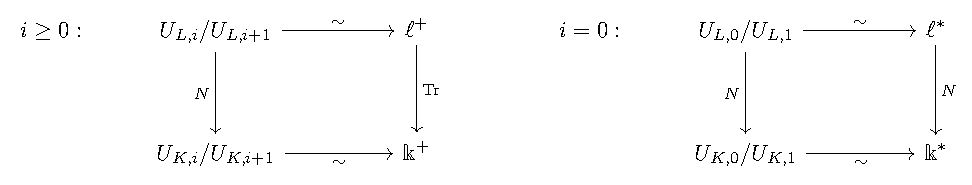
\includegraphics{lectures/6/pictures/cd_24.pdf}
	 \end{center}

	 В них обоих правый столбец сюръективен, а значит, левый тоже. Значит, для $x \in U_k$ можно найти $y \in U_L $ и $x_1 \in U_{K, 1}$ такие, что $x = x_1 \cdot Ny$. Продолжая в том же духе, для $x_1$ мы находим $y_1 \in U_{L, 1}$ и $x_2 \in U_{K, 2}$ такие, что $x_1 = x_2 \cdot Ny$. Соответственно, для $x_m$ мы найдём $y_m \in U_{L, m}$ и $x_{m + 1} \in U_{K, m + 1}$ такие, что $x_m = x_{m + 1} \cdot N y_m$.

	 Заметим, что так как $x_m \in U_{K}^m$, $x_m \xrightarrow{m \to \infty} 1$. Значит, произведение 
	 \[
	 	\prod_{m = 1}^n x_m
	 \]
	 сходится и мы можем перемножить выписанные соотношения на $x_i$ и $y_j$. Перемножая их, мы получаем 
	 \[
	 	x = \Nm(y_1 y_2 \ldots ) \implies \widehat{H}^2(G, U_L) = \widehat{H}^0(G, U_L) = U_k/N U_L = 0.
	 \]

	 Соответственно, отсюда следует, что 
	 \[
	 	\widehat{H}^2(G, U_L) = \widehat{H}^0(G, U_L) = U_K/N U_L = 0.
	 \]

	 Пусть $n = [L : K]$. Заметим, что тогда у нас есть изоморфизм 
	 \[
	 	K^*/NL^* \xrightarrow{\sim} \Z/n\Z, \quad x \mapsto \v_K(x).
	 \]
	 Сначала заметим, что это отображение корректно определено. Действительно,  это следует из формулы
	 \[
	 	\v_L(X) = \frac{\v_K(Nx)}{n} \implies \v_K(Nx) \divby n.
	 \]

	 Проверим, что оно сюръективно. Пусть $\v_K(x) = ns$. Тогда 
	 \[
	  	\v_K\lr*{\frac{x}{\pi^{ns}}} = 0 \implies \frac{x}{\pi^{ns}} \in U_k \implies \frac{x}{\pi^{ns}} \in Ny,
	  \] 
	  где $y \in U_L$ (в последнем переходе мы воспользовались как раз тем, что $H^0(G, U_L) = 0$). Так вот, тогда, так как $\pi^{ns} = N(\pi^s)$, мы получаем $x = N(\pi^s y)$.

	  Таким образом, мы доказали, что $\widehat{H}^{2}(G, L^*) \cong \Z/n\Z$. 

   Дабы не потерять, сформулируем это, как отдельный результат: 

	  \begin{theorem}\label{nerazvetv_H^2} 
	  	Пусть $L/K$~--- конечное неразветвлённое расширение локального поля с группой Галуа $G = \Gal(L/K)$. Тогда $H^2(G, L^*) \cong \mathbb{Z}/n \mathbb{Z}$.
	  \end{theorem}

	  Вообще говоря, для общего развития отметим, что это можно доказать и чисто гомологическими методами в два шага. 

	  \noindent\bf{Шаг 1.} Покажем, что $\widehat{H}^1(G, U_L) = 0$. 

	  Рассмотрим короткую точную последовательность 
	  \[
	  	1 \to U_{L, i + 1} \to U_{L, i} \to U_{L, i}/U_{L, i + 1} \to 1.
	  \]

	  Поскольку $H^{1}(G, U_{L,0}/U_{L, 1}) = H^1(G, \ell^*) = 0$ по теореме Гильберта-90, а $H^1(G, U_{L, i}/U_{L, i + 1}) = 0$, так как $\ell^+$~--- индуцированный модуль \textcolor{red}{Добавить про это комментарий выше под теоремой Гильберта-90!!!}, из длинной точной последовательности пары мы получаем, что для любого коцикла $\varphi \in Z^1(G, U_L)$ найдётся $u \in U_L$ и $\varphi_1 \in Z^1(G, U_L)$ такие, что 
	  \[
	  	\varphi(\sigma) = \frac{\sigma u}{u} \varphi_1(\sigma).
	  \]
	  Дальнейшие действия вполне ясны: 

	  \[
	  	\begin{cases}
	  	 \varphi_1(\sigma) = \frac{\sigma u}{u} \varphi_{1}(\sigma) \\ \vdots \\ \varphi_{m} (\sigma) = \frac{\sigma u_m}{u_m} \varphi_{m + 1}(\sigma) \\ \vdots \\ \end{cases} \implies \varphi(\sigma) = \frac{\sigma(u u _1 \ldots)}{u u_1 u_2\ldots }
	  	 \]

	  	
	  так как $\varphi_m(\sigma) \in U_{L, m}$ и отсюда $\varphi_m(\sigma) \xrightarrow{m \to \infty} 1$. 

	  Таким образом, мы показали, что наш коцикл является кограницей и отсюда заключаем, что $\widetilde{H}^1(G, U_L) \cong 0$.

	  \noindent\bf{Шаг 2.} У нас есть короткая точная последовательность 
	  \[
	  	1 \to U_L \to L^* \xrightarrow{\v_L} \Z \to 0.
	  \]
	  Она индуцирует длинную точную последовательность когомологий: 

	  \begin{center}
	  	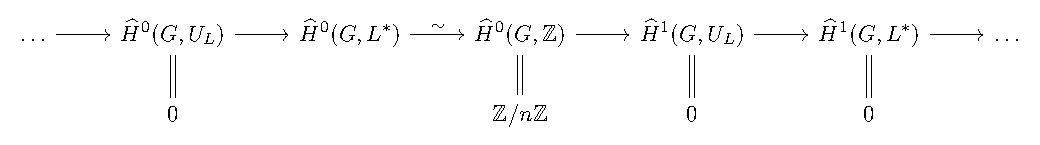
\includegraphics{lectures/6/pictures/cd_25.pdf}
	  \end{center}

	  Ясно, что $\widehat{H}^0(G, \Z) \cong \Z^{G}/ N_{\Z} \Z \cong \Z/n\Z$, так как $N a = |G| a$ (так как действие тривиальное), а $\Z^{G} = \Z$. 

	  Тогда отсюда мы получаем, что $\widehat{H}^{0}(G, \Z) \cong \widehat{H}^0(G, L^*)$, а дальше нужно вновь воспользоваться сдвигом размерности. 

	  \subsubsection{Порядок группы $H^{2}(G, L^*)$ для циклического расширения}

	  Начнем с такого технического результата: 

	  \begin{statement} 
	  	Пусть $L/K$~--- конечное расширение Галуа локального поля с группой Галуа $G = \Gal(L/K)$. Тогда существует такой $G$-подмодуль модуля $U_L$, что 
	  	\begin{itemize}
	  		\item $|U_L/V| < \infty$.
	  		\item $\forall q \ge 1 \quad \widehat{H}^q(G, V) = 0$.
	  	\end{itemize}
	  \end{statement}

	  \begin{proof}
	  	Вспомним теорему о нормальном базисе: если $L/K$~--- расширение Галуа, то существует такой $\alpha \in L$, что $\{ \sigma \alpha \}_{\sigma \in G}$~--- базис $L/K$. Не умаляя общности, можно полагать, что $\alpha \in \cO_{L}$. Рассмотрим $G$-модуль
	  	\[
	  		A = \sum_{\sigma \in G} \cO_{K} \cdot \sigma\alpha \subset \cO_{L}.
	  	\]

	  	Так как $\cO_{L} = \omega_1 \cO_K \oplus \ldots \oplus \omega_n \cO_{K}$ и $\forall i \ \exists N_i \colon \pi^N_{i} \omega_i \in A$, существует $N$ такое, что $\pi^N \cO_{L} \subset A$. Обозначим $M = \pi^{N + 1}A$, тогда 
	  	\[
	  		M \cdot M = \pi^{2N + 2} A \cdot A \subset \pi^{2N + 2} \cO_{L} \subset \pi^{N + 2} A = \pi M
	  	\]
	  	Положим $V = 1 + M \subset U_L$. Заметим, что 
	  	\[
	  		(1 + m_1)(1 + m_2) = 1 + m_1 + m_2 + m_1 m_2 \in 1 + M,
	  	\]
	  	и, кроме того, $V$ замкнут относительно взятия обратного. 

	  	\[
	  		V = 1 + \pi^{N + 1}A \supset 1 + \pi^{2N + 1}\cO_{L} \implies V \subset U_{L, 2N + 1} 
	  	\]
	  	\[
	  		\frac{U_{L}}{U_{L, 2N + 1}} = \frac{U_L}{V} \cdot \frac{V}{U_{L, 2N + 1}},
	  	\]
	  	а так как $|U_L/U_{L, 2N + 1}| < \infty$, отсюда мы получаем, что $|U_{L}/V| < \infty$. 

	  	Тривиальность перывх когомологий с коэффициентами в $U_{L}$ устанавливается таким образом при помощи теоремы о нормальном базисе (которую мы вспоминали в начале доказательства)

	  	\[
	  	 	V_i = 1 + \pi^i M, \quad V = V_0 \supset V_1 \supset V_2 \supset \ldots,
	  	 \] 
	  	 \[
	  	 	V_i/V_{i + 1} \cong M/\pi M \cong \pi^{N+ 1}A/\pi^{N + 2}A \cong A / \pi A = \sum \Bbbk \cdot \sigma \alpha = \Bbbk[G],
	  	 \]
	  	 то есть это индуцированный модуль. Далее нужно действовать полностью аналогично шагу 1 гомологического доказательства теоремы~\ref{nerazvetv_H^2}. Таким образом, $\forall q \ge 1 \ \widehat{H}^q(G, V) = 0$.
	  \end{proof}

	  Пусть теперь $L/K$~---  циклическое расширение локального поля с группой Галуа $G$. Попробуем при помощи доказанного выше предложения понять что-то про порядок группы $H^2(G, L^*)$.

	  Рассмотрим короткую точную последовательность
	  \[
	  	1 \to V \to U_{L} \to U_L/V \to 1.
	  \]

	  Тогда, так как $|U_L/V| < \infty$, по следствию~\ref{Herbran_index_of_finite_module} мы имеем $h(U/V) = 1$. С другой стороны, так как $\widehat{H}^q(G, V) = 0$, $h(V) = 1$. Тогда из короткой точной последовательности выше, пользуясь леммой~\ref{Herbran_calculation} мы заключаем, что $h(U_L) = 1$, что означает, что 
	  \[
	  	|\widehat{H}^0(G, U_L)| = |\widehat{H}^1(G, U_L)|. 
	  \]

	  Рассмотрим теперь другую короткую точную последовательность 
	  \[
	  	1 \to U_L \to L^* \xrightarrow{\v_L} \Z \to 0
	  \]

	  Как мы уже отмечали выше, $\widehat{H}^0(G, \Z)$, а $\widehat{H}^1(G, \Z) \cong \Hom(G, \Z) = 0$, так как группа $G$ конечная. Соответственно, 
	  \[
	  	h(\Z) = \frac{|\widehat{H}^0(G, \Z)|}{|\widehat{H}^1(G, \Z)|} = \frac{|\Z/n\Z|}{|\Hom_{\Grp}(G, \Z)|} = \frac{n}{1} = n.
	  \]
	  Тогда из точной последовательности выше по лемме~\ref{Herbran_calculation} мы получаем, что 
	  \[
	  	h(L^*) = h(U_L) \cdot h(\Z) = 1 \cdot n = n.
	  \]
	  С другой стороны, пользуясь периодичность когомологий Тейта для циклической группы
	  \[
	  		h(L^*) = \frac{|\widehat{H}^0(G, L^*)|}{|\widehat{H}^1(G, L^*)|} = \frac{|\widehat{H}^2(G, L^*)|}{1} = |\widehat{H}^2(G, L^*)|
	  \]

	  Таким образом, мы доказали такую теорему. 

	  \begin{theorem} 
	  	Пусть $L/K$~--- циклическое расширение локального поля $K$ степени $n$ с группой Галуа $G = \Gal(L/K)$.  Тогда $|\widehat{H}^2(G, L^*)| = n$. 
	  \end{theorem}

	  
